\chapter{Descripción del sistema mecánico}
\label{ch:problema}
\section{Componentes y transmisión de cargas}
Un aerogenerador de eje horizontal combina una estructura portante casi estacionaria con un conjunto rotor que desarrolla un movimiento de gran amplitud. La torre transmite las acciones a la cimentación; la góndola aloja componentes que se idealizan mediante masas y tensores de inercia; el cubo transmite acciones entre el eje y las tres palas. La velocidad angular del rotor no mide la deformación de las palas: una pala puede completar numerosas revoluciones sin deformarse, y también puede flexionar durante ese movimiento. El modelo debe separar ambos fenómenos antes de introducir las ecuaciones dinámicas.

La torre y las palas se representan como cuerpos deformables unidimensionales, mientras que la góndola y el conjunto cubo--nariz se describen como cuerpos rígidos. Las conexiones transmiten fuerzas y momentos de acuerdo con sus restricciones cinemáticas o sus leyes elásticas. Esta idealización conserva la respuesta estructural global y permite expresar de forma explícita la contribución de cada componente a las ecuaciones del sistema.

\begin{figure}[htbp]
\centering
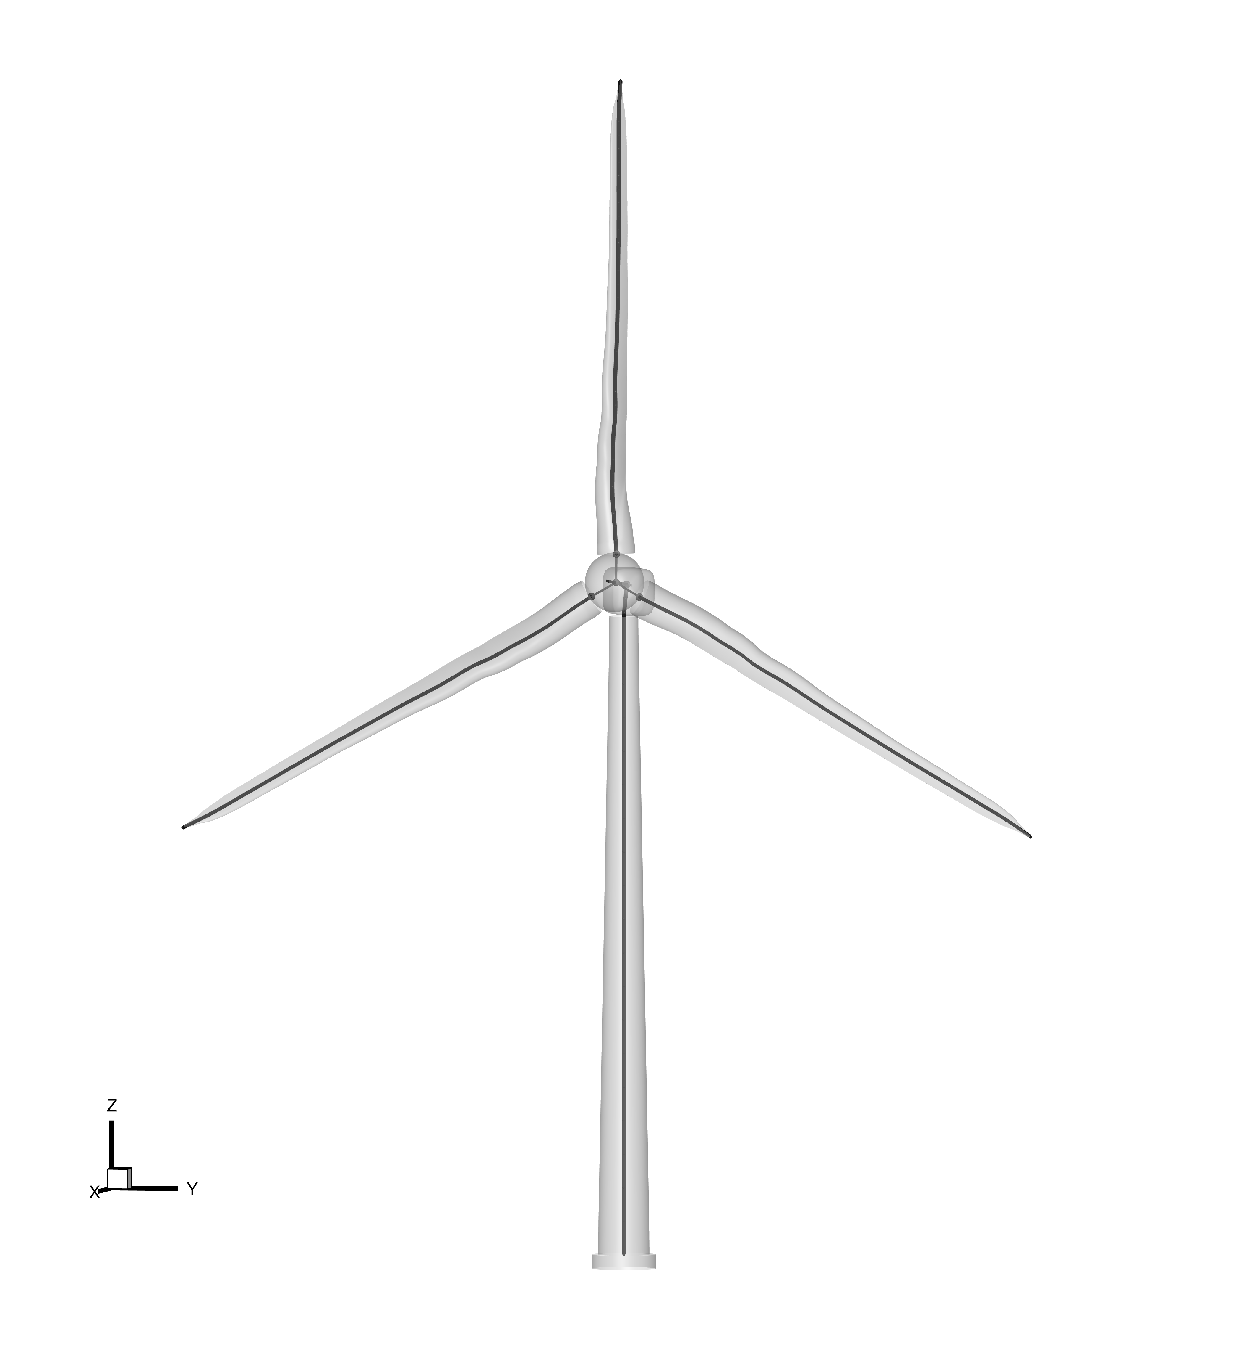
\includegraphics[width=.96\linewidth,height=.50\textheight,keepaspectratio]{figures/tecplot/turbina_3d.pdf}
\caption[Componentes del aerogenerador y eje nominal del rotor]{Vista tridimensional del aerogenerador y su idealización estructural. Las líneas y los nodos interiores corresponden a las vigas del modelo existente; las envolventes de torre, palas, góndola y cubo facilitan su identificación. Los perfiles de pala y las carcasas son ilustrativos: no proceden de un modelo CAD ni de una discretización de sólidos. Se conservan las coordenadas nodales y la conectividad del modelo.}\label{fig:turbina}
\end{figure}

\begin{figure}[htbp]
\centering
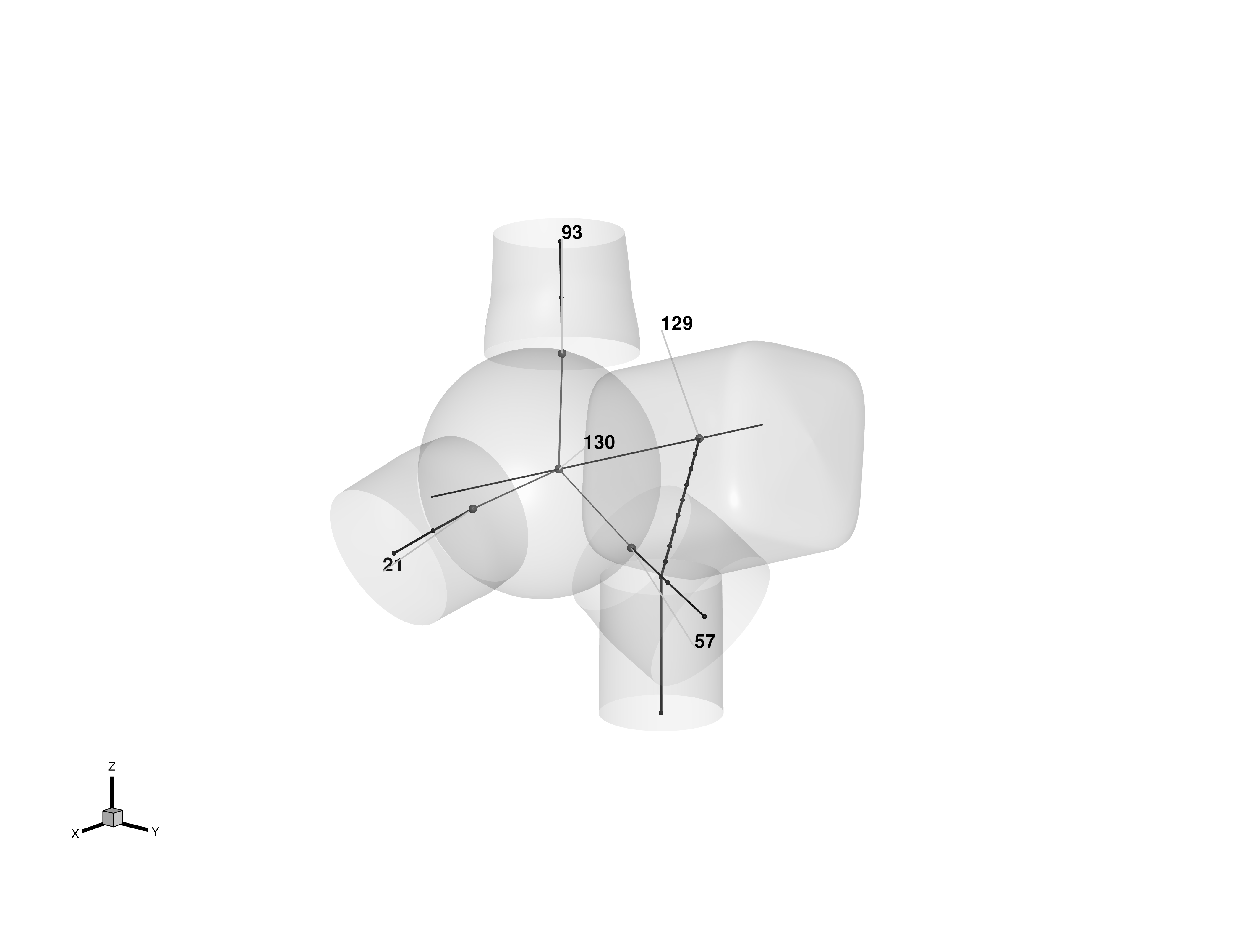
\includegraphics[width=.94\linewidth,height=.38\textheight,keepaspectratio]{figures/tecplot/turbina_conexiones_3d.pdf}
\caption[Conexiones interiores del rotor]{Detalle espacial de los elementos unidimensionales dentro de la envolvente del rotor. Se identifican los nodos de góndola 129, cubo 130 y raíces 21, 57 y 93. Las relaciones de raíz se imponen mediante compatibilidad cinemática; las envolventes son ilustrativas.}
\label{fig:conexiones3d}
\end{figure}


\section{Idealizaciones de los componentes}
La torre y cada pala se modelan mediante una línea de referencia y un triedro de sección. Las secciones pueden trasladarse y rotar; se admite deformación axial, cortante, torsión y flexión en dos planos. Esta descripción es de tipo Timoshenko en su especialización lineal. Que la sección sea rígida en su plano no significa que toda la viga sea rígida: la variación de posición y orientación de una sección a otra produce deformación.

La góndola y el conjunto cubo--nariz se idealizan como cuerpos rígidos diferentes. Cada uno posee masa, centro de masa y tensor de inercia propios. La sección superior de la torre se conecta a la góndola, y la unión entre la góndola y el cubo se representa mediante una ley elástica para los movimientos relativos de perturbación. Las raíces de las palas quedan unidas rígidamente al cubo, con la separación geométrica definida por sus brazos de conexión. El giro nominal del rotor se prescribe independientemente de estas perturbaciones.

En la presente descripción, la base sigue una traslación conocida y no una rotación impuesta. Una cimentación flexible puede representarse mediante relaciones adicionales entre acciones y desplazamientos. Sin embargo, un resorte equivalente no constituye por sí mismo un modelo continuo del suelo ni identifica sus propiedades. Para estudiar el suelo como cuerpo deformable sería necesario añadir su dominio, cinemática y ley constitutiva.

\section{Movimiento nominal y excitaciones}
La velocidad de operación se prescribe por
\begin{equation}
 \psi(t)=\psi_0+\Omega t,\qquad \dot\psi=\Omega,\qquad \ddot\psi=0.
 \label{eq:psi}
\end{equation}
El ángulo $\psi$ puede crecer sin límite; la aproximación de pequeña perturbación no se aplica a ese ángulo. La velocidad $\Omega$ tiene unidades de $\mathrm{rad/s}$ y es un dato, no una incógnita obtenida del equilibrio de pares. Si se proporciona una velocidad $n$ en revoluciones por minuto, $\Omega=2\pi n/60$.

Una \emph{operación prescrita} significa que se impone la evolución de una variable cinemática. El par necesario para mantenerla puede ser distinto de cero. El motor, generador o mecanismo ideal que sostiene el giro suministra o extrae la potencia requerida, aunque su dinámica de control no se resuelva. Por tanto, prescribir velocidad no equivale a imponer ausencia de acciones en el eje.

La dirección nominal del viento se considera fija y el eje del rotor permanece alineado con ella. La góndola mantiene una orientación nominal constante; por tanto, el movimiento de guiñada no forma parte de la operación prescrita. Las variaciones de velocidad del viento se representan mediante las cargas externas. Las pequeñas rotaciones estructurales de la góndola y el cubo pertenecen a la respuesta vibratoria y se distinguen de una maniobra de orientación.

La excitación sísmica se describe mediante una traslación conocida de la base. Las cargas aerodinámicas se introducen como fuerzas y momentos distribuidos sobre la torre y las palas. Su expresión admite dependencia de la configuración, de la velocidad estructural y del tiempo. La formulación estructural utiliza estas acciones y sus derivadas respecto del estado; un cálculo acoplado del flujo requiere, adicionalmente, las ecuaciones y condiciones de contorno del problema aerodinámico.

\section{Hipótesis de la representación estructural}
Los componentes se describen en un espacio euclídeo tridimensional. La torre y las palas se consideran esbeltas, de modo que su respuesta global puede representarse mediante variables definidas sobre una línea y propiedades integradas en la sección transversal. Quedan fuera de esta representación los fenómenos locales de pared, la delaminación y las concentraciones tridimensionales de tensiones en las uniones.

La cinemática se establece con rotaciones finitas para conservar exactamente el giro nominal. Las vibraciones se describen mediante pequeñas perturbaciones respecto del estado de operación, y las deformaciones elásticas se suponen pequeñas. Esta distinción permite que una pala complete una revolución sin aplicar la aproximación de ángulo pequeño a su azimut. La aproximación lineal se refiere al movimiento relativo de deformación, no a la trayectoria absoluta.

La geometría de referencia especifica la forma y orientación inicial de las secciones. Sus variaciones, la curvatura inicial y la torsión geométrica se describen mediante las propiedades y orientaciones de los tramos. El paso de pala y el ángulo de cono son constantes cuando pertenecen a la geometría de montaje. Los elementos rectos aproximan esta geometría por segmentos, conservando las conexiones entre componentes.
